\documentclass[journal]{IEEEtran}
\usepackage{xcolor,soul,framed}
\usepackage[cmex10]{amsmath}
\usepackage{amssymb}
\usepackage{tikz}
\usetikzlibrary{positioning}

\newcommand{\xx}{\textbf{x}}

\newcommand{\yy}{\textbf{y}}

\begin{document}

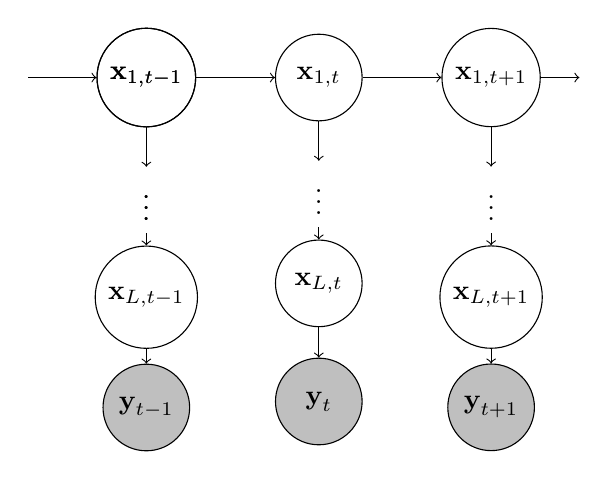
\begin{tikzpicture}
[
roundnode/.style={circle, draw=black, minimum size=1.1 cm},
squarednode/.style={rectangle, draw=black,  minimum size=5mm},
dot/.style={circle, draw=white,  minimum size=0.7cm},
]
%Nodes
\node[roundnode]   (point)    {$\xx_{1, t-1}$};
\node[dot]         (p2)        [below=0.5cm of point] {$\vdots$};

\node[roundnode]   (point)    {$\xx_{1, t-1}$};
\node[dot]         (p2)        [below=0.5cm of point] {$\vdots$};
\node[roundnode]     (p3)     [below=1.5cm of point] {$\xx_{L, t-1}$};
\node[roundnode,fill=lightgray]     (p4)     [below=3cm of point] {$\yy_{t-1}$};

\node[roundnode]     (q1)       [right=of point] {$\xx_{1, t}$};
\node[dot]            (q2)      [below=0.5cm of q1] {$\vdots$};
\node[roundnode]      (q3)     [below=1.5cm of q1] {$\xx_{L, t}$};
\node[roundnode,fill=lightgray]      (q4)    [below=3cm of q1] {$\yy_{t}$};

\node[roundnode]     (r1)    [right=of q1] {$\xx_{1, t+1}$};
\node[dot]           (r2)    [below=0.5cm of r1] {$\vdots$};
\node[roundnode]     (r3)    [below=1.5cm of r1] {$\xx_{L, t+1}$};
\node[roundnode,fill=lightgray]     (r4)    [below=3cm of r1] {$\yy_{t+1}$};

%Lines
\draw[->] (point.south) -- (p2.north);
\draw[->] (p2.south) -- (p3.north);
\draw[->] (p3.south) -- (p4.north);

\draw[->] (point.east) -- (q1.west);

\draw[->] (q1.south) -- (q2.north);
\draw[->] (q2.south) -- (q3.north);
\draw[->] (q3.south) -- (q4.north);

\draw[->] (q1.east) -- (r1.west);

\draw[->] (r1.south) -- (r2.north);
\draw[->] (r2.south) -- (r3.north);
\draw[->] (r3.south) -- (r4.north);
\draw[->] (r1.east) -- (5.5, 0);
\draw[->] (-1.5, 0) -- (point.west);
\end{tikzpicture}

\end{document}